% !TEX root = main.tex
\newpage
\section{Experiments} \label{sec:experiments}
\subsection{Image Classification}

Training a binary classifier with imbalanced data is a challenging task in machine learning. Practices for dealing with imbalance include optimizing class weight hyperparameters, hard negative mining \citep{shrivastava2016training} and synthetic minority oversampling \citep{chawla2002smote}. 
Without accounting for imbalance, the minority samples are often misclassified in early stages of the iterative training procedures, resulting in high loss and high gradient norms associated with these points. Importance sampling schemes for reducing the variance of the gradient norms will sample these instances more often at the early phases, offering a way of tackling imbalance.

For verifying this intuition, we perform the image classification experiment of \cite{bouchard2015online}. We train one-vs-all logistic regression Pascal VOC 2007 dataset \citep{everingham2010pascal} with image features extracted from the last layer of the VGG16 \citep{simonyan2014very} pretrained on Imagenet. We measure the average precision by reporting its mean over the 20 classes of the test data. The optimization is performed with AdaGrad \citep{duchi2011adaptive}, where learning rate is initialized to 0.1. The losses received by the bandit methods are the norms of the logistic loss gradient.
We compare our method, Variance Reducer Bandit (VRB), to:
\vspace{-1.5mm}
\begin{itemize}
\setlength\itemsep{0.05em}
\item uniform sampling for SGD,
\item Adaptive Weighted SGD (AW) \citep{bouchard2015online} ---  variance reduction by sampling from a chosen distribution whose parameters are optimized alternatingly with the model parameters,
\item MABS \citep{salehi2017} --- bandit algorithm for variance reduction that relies on EXP3 through employing modifies losses.  
\end{itemize}

\begin{figure}[h]
\centering
\begin{minipage}{.48\textwidth}
  \centering
  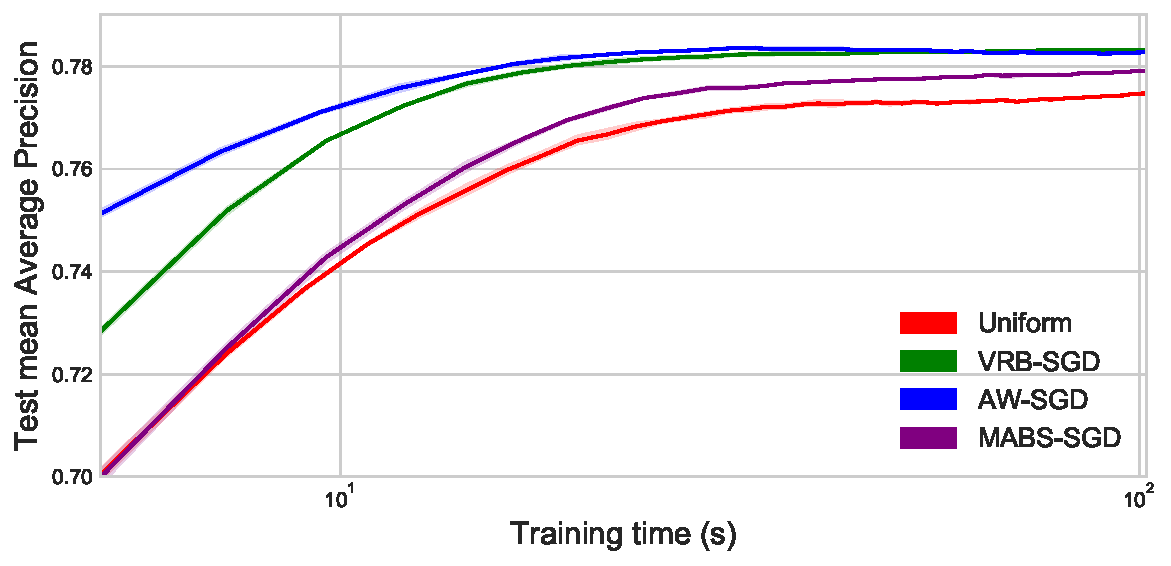
\includegraphics[width=\linewidth]{figures/voc-result.pdf}
      \caption{Mean Average Precisions on the test part of VOC 2007.}
      \label{fig:voc-results}
\end{minipage}%
\quad
\begin{minipage}{.48\textwidth}
  \centering
  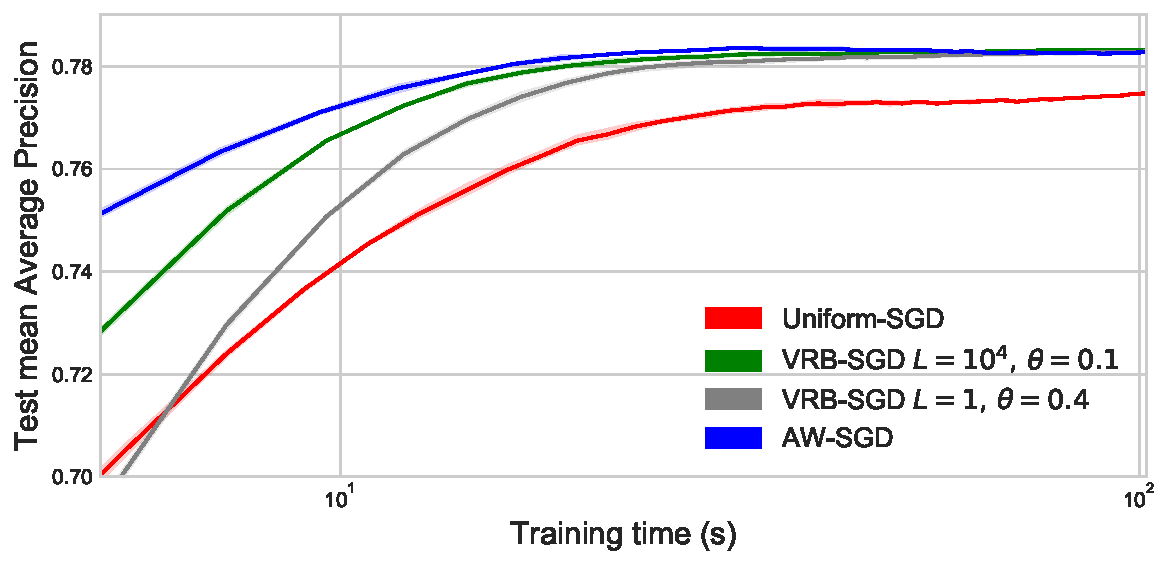
\includegraphics[width=\linewidth]{figures/voc-result-2.pdf}
      \caption{The effect of different hyperparameters on VRB. }
      \label{fig:voc-results-2}
\label{fig:test}
\end{minipage}%
\end{figure}

        
The hyperparameters of the methods are chosen based on cross-validation on the validation portion of the dataset. The results can be seen in Figure \ref{fig:voc-results}, where the shaded areas represent confidence $95\%$ intervals over 10 runs. The best performing method is AW, but its disadvantage compared to the bandit algorithms is that it requires choosing a family of sampling distributions, which usually incorporates prior knowledge, and calculating the derivative of the log-density. VRB and AW both outperform uniform subsampling with respect to the training time.  VRB performs similarly to AW at convergence, and speeds up training 10 times compared to uniform sampling, by attaining a certain score level 10 times faster. We have also experimented with the variance reduction method of \cite{pmlr-v70-namkoong17a}, but it did not outperform uniform sampling significantly. Since cross-validation is costly, in Figure \ref{fig:voc-results-2} we show the effect of the hyperparameters of our method. More specifically, we compare the performance of VRB with misspecified regularizer $L=1$ to the best $L=10^8$ chosen by cross-validation, and we compensate by using higher mixing coefficient $\theta=0.4$. The fact that only the early-stage performance is affected is a sign of method's robustness against regularizer misspecification.

We also measure the regret incurred both by the full information and VRB samplers, and show the results in Figure \ref{fig:regret}. For a fair comparison, we choose an \emph{oblivious} adversary that generates the loss sequences by performing the same optimization process as described above on a subset of 1000 data points from VOC 2007, with uniform sampling. For VRB, we report the average regret over 10 runs. 
\begin{figure}[h]

		\centering
		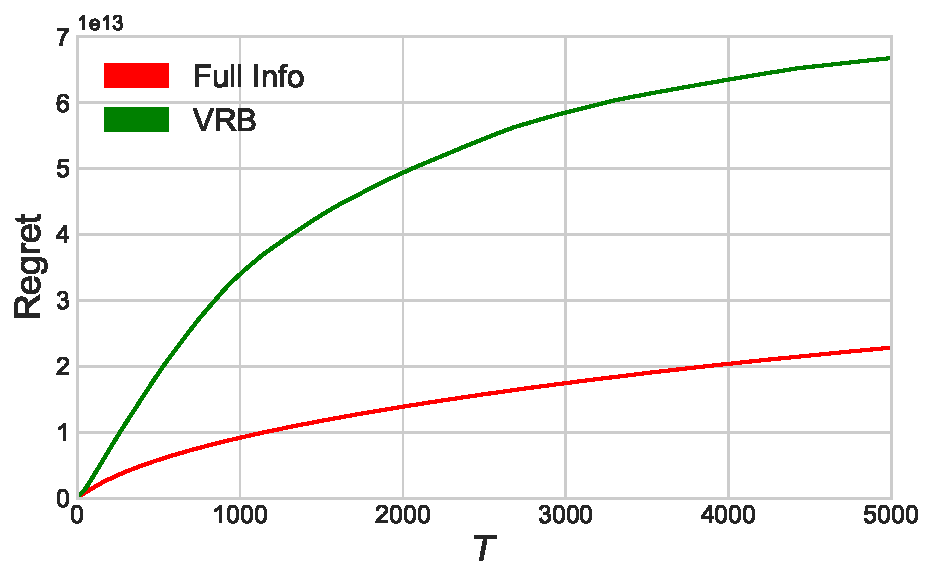
\includegraphics[width=0.5\linewidth]{figures/regret.pdf}
		\caption{Regret incurred by the full info and VRB.}
		\label{fig:regret}
\end{figure}


\subsection{$k$-Means}

In this experiment, we show that in some applications it is beneficial to work with per-sample upper bound estimates $L_i$ instead of a single global bound. As an illustrative example, we choose mini-batch $k$-Means clustering \citep{sculley2010web}. This is a slight deviation from the presented theory, since we sample multiple points for the batch and update the sampler only  once, upon observing the loss for the batch. 

In the case of $k$-Means, the parameters consist of the coordinates of the $k$ centers \linebreak $Q=\{q_1, q_2, \dots, q_k\}$. As the cost function for a point $x_i \in \{x_1, x_2, \dots, x_n \}$ is the  squared Euclidean distance to the closest center, the loss received by VRB  is the norm of the gradient  \linebreak $\min _{q \in Q } 2 \cdot || x_i - q||_2$. This lends itself to a natural estimation of $L_i$:
choose a point $u$ randomly from the dataset and define $L_i=4 \cdot || x_i - u||^2_2$. For this experiment, we set $\theta=0.5$.

We solve mini-batch $k$-Means  for $k=100$ and batch size $b=100$ with uniform sampling and VRB. The initial centers are chosen with $k$-Means++ \citep{arthur2007k} from a random subsample of 1000 points from the training data and they are shared between the methods. We generate 10 different sets of initial centers and run both algorithms 10 times on each set of centers, with different random seeds for the samplers.  We train the algorithm on $80 \%$ of the data, and measure the cost of the $20 \%$ test portion for the following datasets:
\vspace{-2mm}
\begin{itemize}
\setlength\itemsep{0.2em}
  \item \texttt{CSN} \citep{faulkner2011next} --- cellphone accelerometer with 80,000 observations and 17 features,
 \item \texttt{KDD} \citep{kddcup2004} --- data set used for Protein Homology Prediction KDD
    competition  containing 145,751 observations with 74 features,
    \item \texttt{MNIST} \citep{lecun1998gradient} --- 70,000 low resolution images of handwritten
    characters transformed using PCA with whitening and retaining 10 dimensions.  
\end{itemize}

\begin{figure}[h]
      \centering
      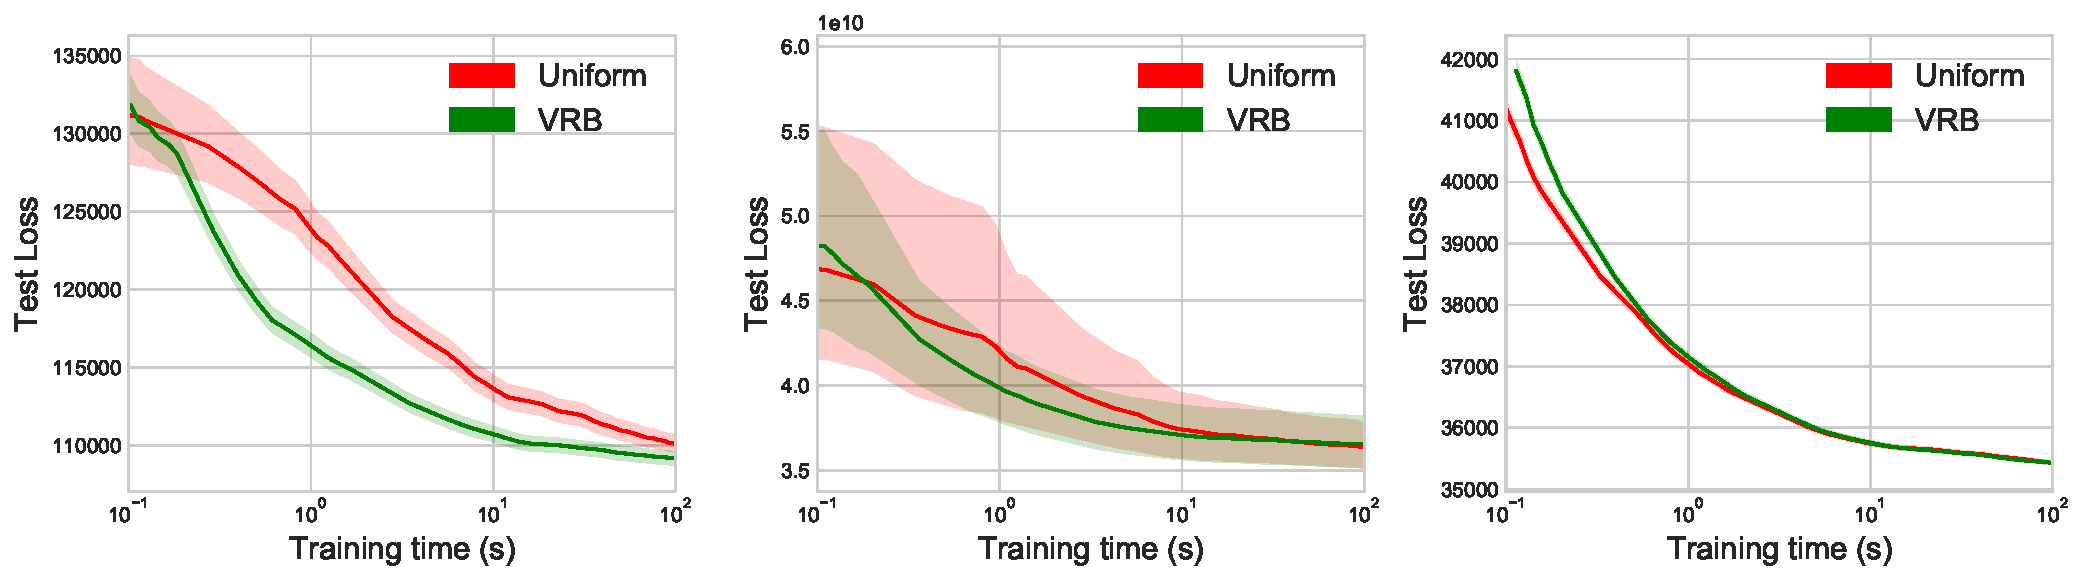
\includegraphics[width=\linewidth]{figures/kmeans.pdf}
      \caption{The evolution of the loss of $k$-Means on the test set. The shaded areas represent $95\%$ confidence intervals over 100 runs.}
      \label{fig:kmeans-results}
        \end{figure}
        
The evolution of the cost function on the test set with respect to the elapsed training time is shown in Figure \ref{fig:kmeans-results}. The chosen datasets illustrate three observed behaviors of our algorithm. In the case of \texttt{CSN}, our method significantly outperforms uniform subsampling. In the case of \texttt{KDD}, the advantage of our method can be seen in the reduced variance of the cost over multiple runs, whereas on \texttt{MNIST} we observe no advantage.
This behavior is highly dependent on intrinsic dataset characteristics: for \texttt{MNIST}, we note that the entropy of the best-in-hindsight sampling distribution is close the entropy of the uniform distribution. We have also compared VRB with the bandit algorithms mentioned in the previous section. Since mini-batch $k$-Means converges in 1-2 epochs, these methods with  uniform initialization do not outperform uniform subsampling significantly. Thus, for this setting, careful initialization is necessary, which is naturally supported by our method.
